\section{Topology Generator for Federated IT Networks\label{sec:topologies.approach}}

To solve the limitations of existing datasets in the literature, we introduce \thecontrib, a topology generator for federated IT networks.
In this section, we present the design and architecture of \thecontrib, before detailing its implementation using Airbus' CyberRange platform\footnote{\url{https://www.cyber.airbus.com/products/cyberrange/}}.
While \thecontrib is not released as an open-source tool yet, the code is available upon request.


\subsection{Approach Overview\label{sec:topologies.approach.overview}}

The core idea behind \thecontrib is to compose network topologies by selecting and connecting a set of predefined sub-topologies that satisfy user-supplied constraints.
A sub-topology is a small network composed of a subnet, a set of nodes (clients or servers), and a gateway that connects the subnet to the rest of the network.
We build a library of sub-topologies that represent common network configurations.
While creating this library remains human operated, the composition of the topologies is fully automated, allowing the generation of different topologies with common characteristics.

\thecontrib is a thus two-step algorithm:
\begin{enumerate}
  \item \emph{Topology selection:} Use constraint programming to find all sets of sub-topologies that satisfy the user-defined constraints, based on a library of predefined sub-topologies.
  \item \emph{Topology composition:} For each set, connect the sub-topologies in a random tree-like structure starting from the \emph{Master} sub-topology.
\end{enumerate}

\begin{figure}[t]
  \centering
  \begin{subfigure}[b]{0.34\linewidth}
    \centering
    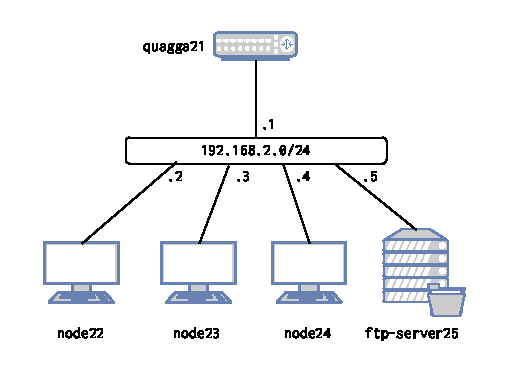
\includegraphics[width=\linewidth]{figures/sub_topology.pdf}
    \caption{
      Example of a sub-topology containing 3 Windows clients and 1 FTP server.
      %The node labeled \texttt{quagga21} is the gateway connecting the sub-topology to the rest of the network.
      \label{fig:topologies.example}
    }
  \end{subfigure}
  \hfill
  \begin{subfigure}[b]{0.64\linewidth}
    \centering
    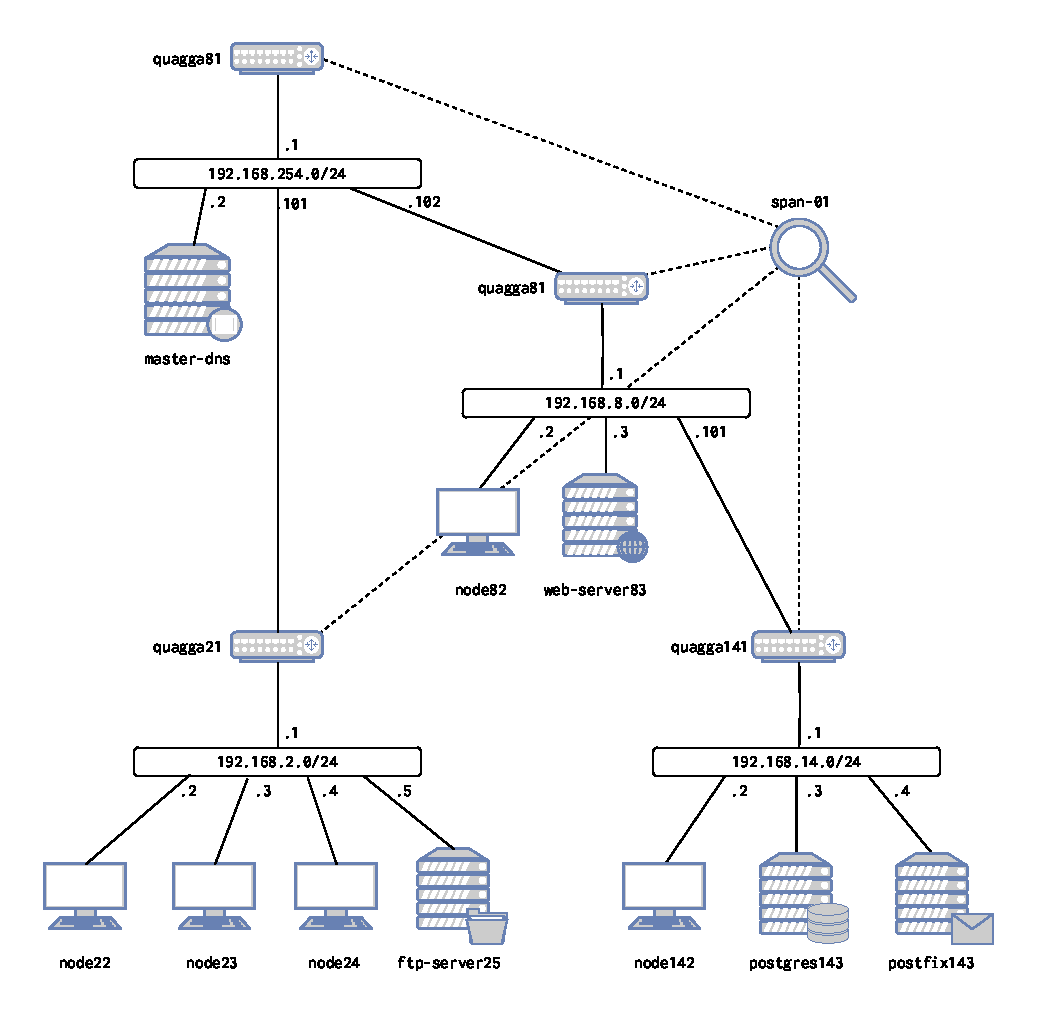
\includegraphics[width=\linewidth]{figures/topology.pdf}
    \caption{
      Example of a complete topology composed of 3 sub-topologies.
      The \texttt{span} captures the traffic of all gateways to simulate various probe positions afterward.
      \label{fig:topologies.topology}
    }
  \end{subfigure}
  \caption{
    Examples of topologies as instantiated on Airbus' CyberRange.
    Each node represents a machine, and the edges represent the connections between them.
    Nodes labeled \texttt{quagga*} are gateways connecting each sub-topology to the rest of the network.
  }
\end{figure}


\subsubsection{Topology selection}

The topology selection is the most important part of the algorithm, as it requires finding all sets of sub-topologies that satisfy the user-defined constraints.
A sub-topology is composed of a subnet, a set of nodes (clients or servers), and a gateway that connects the subnet to the rest of the network.
\Cref{fig:topologies.example} shows an example of a sub-topology with 4 nodes.
The gateway $g_x$ is a particular node (not comprised in $N_x$) that connects the subnet to the rest of the network.
A sub-topology can therefore be represented as a tuple $t_x = ( x, N_x, g_x )$.
Selecting sub-topologies from the library is a \gls{csp} which aims at finding all sets of sub-topologies that satisfy the user-defined constraints.
\Cref{def:csp} defines the concept of a \gls{csp}.

\begin{definitionbox}{\acrfull{csp}~\normalfont\cite{russell_Artificialintelligencemodern_2021}}{csp}
  A \acrfull{csp} is a tuple $P = ( X, D, C )$ where:
  \begin{itemize}
    \item $X = ( X_1, X_2, \ldots, X_n )$ is a set of variables.
    \item $D = ( D_1, D_2, \ldots, D_n )$ is a set of non-empty domains, one for each variable.
    \item $C = ( C_1, C_2, \ldots, C_n )$ is a set of constraints that specify allowable combinations of values in their domains.
  \end{itemize}

  Each constraint $C_j \in C$ is a new tuple $C_j = ( \chi, R )$ where $R$ is a relation between the variables in $\chi \subseteq X$.
  Thus, solving a \gls{csp} is finding an assignment of values from $X$ in $D$ that satisfies all constraints in $C$.
\end{definitionbox}



While dimensioning the output topologies can easily be translated using numeric boundaries, the constraints on the availability of services and attack scenarios in the sub-topologies are slightly more challenging.
We first define the service domain $D_\text{service}$ as the set of all services available in the library of sub-topologies, and tag each service node with its corresponding name, such as \texttt{ftp}, \texttt{postfix} (for email), or \texttt{ldap}.
An attack scenario is defined as another tuple $a_k = ( \text{srcs} = \{N_1, N_2, \ldots\}, \text{targets} = \{N_{11}, N_{12}, \ldots\} ) $ where \texttt{srcs} and \texttt{targets} are sets of nodes available in the library that are compatible with the attack scenario.
For instance, a \gls{mitm} attack could be represented as $a_\text{MitM} = ( \text{srcs} = \lbrace N_\text{attaker} \rbrace, \text{targets} = \lbrace N_1, N_2 \rbrace ) $.
Based on the aforementioned definitions, we can define our \gls{stsp} in \Cref{def:stsp}.

\begin{problembox}{\Acrfull{stsp}}{stsp}
  Let $T = \{t_1, t_2, \ldots, t_n\}$ be a set of sub-topologies, $D_\text{service}$ a set of services, $A = \{a_1, a_2, \ldots, a_m\}$ a set of attack scenarios, $n_\text{min}$ and $n_\text{max}$ the bounds of the number of subtopologies, and $h_\text{min}$ and $h_\text{max}$ the bounds for the total number of nodes.
  Find all sets of sub-topologies $T' \subseteq T$ that satisfy the following:
  \begin{enumerate}
    \normalfont
    \item $n_\text{min} \leq \#T' \leq n_\text{max}$.
    \item $h_\text{min} \leq \sum\nolimits_{t_s \in T'} \#N_s \leq h_\text{max}$.
    \item $\forall s \in D_\text{service}, \exists t_s \in T', s \in N_s$.
    \item $\forall a \in A, \forall \emph{src} \in a_{[\emph{srcs}]}, \exists t_s \in T', \emph{src} \text{ compatible with } t_s$.
    \item $\forall a \in A, \forall \emph{target} \in a_{[\emph{targets}]}, \exists t_s \in T', \emph{target} \text{ compatible with } t_s$.
    % \item The number of sub-topologies in $T'$ is between $n_\text{min}$ and $n_\text{max}$.
    % \item The total number of nodes in $T'$ is between $h_\text{min}$ and $h_\text{max}$. 
    % \item Each service in $D_\text{service}$ is available in at least one sub-topology in $T'$.
    % \item Each attack scenario in $A$ is compatible with at least one sub-topology in $T'$.
  \end{enumerate}
\end{problembox}


\subsubsection{Topology composition}

Once the sub-topologies are selected, the next step is to connect them to form a complete IT network.
The composition of the topologies is done in a tree-like structure, starting from the \emph{Master} sub-topology.
The \emph{Master} sub-topology is a special sub-topology that acts as the root of the tree and contains the necessary services to route traffic between the sub-topologies.
\Cref{fig:topologies.topology} shows an example of a complete topology composed of 3 sub-topologies.
At this point of the algorithm, the sub-topologies are already selected, and the composition is a simple matter of connecting the gateways while respecting the last constraint of tree-depth.
Yet, many variations of the same tree can be created, as illustrated in \Cref{fig:topologies.trees}.

\begin{figure}
  \centering
  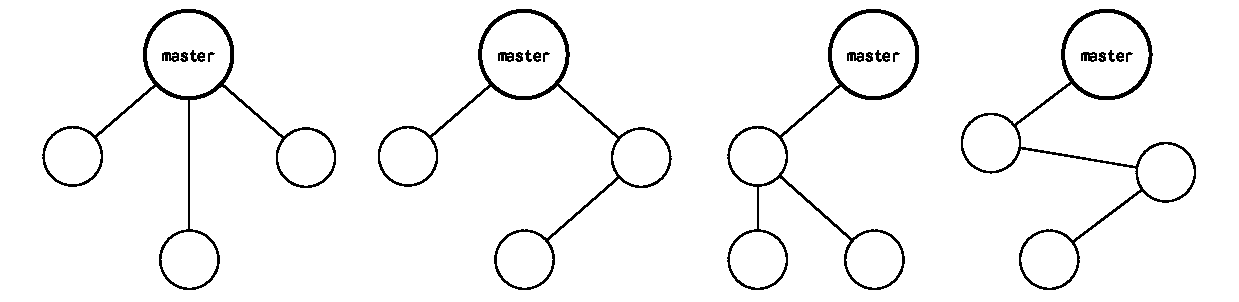
\includegraphics[width=0.9\linewidth]{figures/trees-3.pdf}
  \caption{
    Possible unlabeled tree structures for a topology composed of 3 sub-topologies.
    The biggest node represents the \emph{Master} sub-topology.
    \label{fig:topologies.trees}
  }
\end{figure}

\subsection{Implementation\label{sec:topologies.approach.implementation}}

In this section, we present parts of the implementation of \thecontrib using Airbus' CyberRange platform.
A CyberRange is a virtual environment that simulates a real-world network, allowing users to train and test their cybersecurity skills.
Most importantly, such platforms come with a set of templates that can be used to create sub-topologies, and compatible attack scenarios and user traffic generation tools to generate realistic traffic.
We implement our topology generator as a Python script that interacts with the CyberRange platform through its API to query the available sub-topologies, services, and attack scenarios.
The topology-selection algorithm is implemented using Google's \texttt{CP-SAT} solver\footnote{\url{https://developers.google.com/optimization/cp/cp_solver}}, and we develop a simple recursive algorithm to compose the topologies.
The constraints on the availability of services and attack scenarios are implemented as a simple filtering algorithm that removes sub-topologies that do not contain the required services or are not compatible with the attack scenarios.
We seed all random operation to ensure deterministic results.


\paragraph{The \emph{Master} sub-topology.}

The \emph{Master} topology serves as the basis for the composition.
It consists of a gateway connecting it to the Internet, a DHCP server for distributing IP addresses, and a DNS server for resolving domain names across all topologies.
This is the only topology that receives manual configuration.
We set up the DNS server to associate domain names to the IPs of the services hosted in the sub-topologies: \eg, web server (\texttt{webserver.local}), mail server (\texttt{mailserver.local}), file sharing (\texttt{fileserver.local}).
This approach makes it possible to define unique domain names for each service, and make them accessible from any sub-topology.


\paragraph{Handling connectivity.}

Now that all services are available using their domain names, the next step is to ensure that the services are reachable from any sub-topology.
To do so, each gateway $g_s$ hosts a DHCP server with a dedicated range to allocate IP addresses for its child sub-topologies.
The DNS configuration of the \emph{Master} topology is propagated to the DHCP server of each gateway, so that the domain names are resolved correctly.
To route traffic between the sub-topologies, the gateways also run an OSPF daemon to exchange routing information, announcing their own subnet to the rest of the network.
This setup allows to dynamically configure the routing tables of the sub-topologies upon deployment, and ensures that all machines are reachable.


\paragraph{Constraint satisfaction.}

As noted in \Cref{sec:topologies.approach.overview}, the topology selection is a \gls{csp} that can be solved using a constraint solver.
In particular, we implement our cardinality-related constrains (\ie, the number of sub-topologies and nodes) using Google's \texttt{CP-SAT} solver.
This generates all possible combinations of sub-topologies that satisfy the numeric constraints.
We then prune the sets that do not contain the required services or are not compatible with the attack scenarios.
For each set, we compose the complete topology using a simple recursive algorithm that connects the gateways of the sub-topologies in a tree-like structure, starting from the \emph{Master} sub-topology.
The algorithm includes a backtracking mechanism to roll back the composition when the tree-depth constraint is not satisfied, and try again from another branch.